% #############################################################################
% This is Chapter 6
% !TEX root = ../main.tex
% #############################################################################
% Change the Name of the Chapter i the following line
\fancychapter{System Evaluation}
\cleardoublepage
% The following line allows to ref this chapter
\label{chap:evaluation}

This chapter concerns the system and board evaluation. The system and board were evaluated regarding its performance and the fullfilled requirements outlined in the previous project report and the problem definition chapter \ref{chap:problem}.
% -----------------------------------------------------
% -----------------------------------------------------
\section{Performance Tests}\label{chap:evaluation:performance}

The test objectives, configuration, results and conclusions are detailed for every tested component.
The communication channel, smartfusion2 board's security services and implemented services were tested.
Two performance metrics were calculated, the test processing time, and the tested component's throughput.

% -----------------------------------------------------
\subsection{Testing configuration}\label{chap:evaluation:performance:config}

The tests were all performed on a Windows 10 computer, connected to the smartfusion2 device through a \ac{UART} serial port. The implemented PKCS\#11 program interface was used to run the tests.
Two programs were running on the computer while performing the tests, the PKCS\#11 interface program and the SoftConsole IDE to run the code on the smartfusion board.
For all tests, the serial port UART connection was configured with a 115200 bit/s baud rate.%, 8 data bits, no parity bits and one stop bit.
Since the board does not provide a clock and \ac{API} to measure elapsed time, the time has to be measured in the interface software side.
The elapsed time was measured using the function \texttt{gettimeofday()} available in the C library \texttt{sys/time.h}.
Time measurement starts right before sending a message to the device which triggers the operation, and stops when the client receives a message from the device, after the operation is finished.
In order to thoroughly study the performance and scalability of each component, the transmitted data size was varied, only for components where it is logical and can potentially have a performance impact. The data size was tested, when possible, up to 36 KBytes. The size is limited by the device's \ac{RAM} of 64 KB.
Tests were performed in two different configurations.
Obvious outlier values were excluded from the experimental calculations. The adopted rule was that values which are significantly above or below the average, and are never repeated were eliminated from the sample set.
For the first test configuration, the measured operation is performed once in the device each transmission. This transmission is repeated multiple times, minimum thirty, for each set of values, until an acceptable variance is achieved. For most components the variance is well bellow 1\%. % The more volatile test results have a variance below 4\%.
For most components the first configuration produced unstable results with a high variance, due to the communications overhead on every test run.
Thus, a second test configuration was applied on components where the time to transmit messages needs to be minimized to more accurately assess its performance. For each transmission, the operation was performed 100 consecutive times in the board. The resulting time was divided by 100 to obtain the average processing time of the operation.
With the second configuration, the tests are visibly more stable.
A test example of the difference between both configurations results was on testing the \ac{AES} security service. The first scenario's communication overhead was on average 15\% compared to the second configuration results, with a peak 61\% overhead for small data sizes. Additionally when plotting the results, the second results scale almost perfectly linear, and the first results' are significantly more unstable.

% -----------------------------------------------------
\subsection{Communications}\label{chap:evaluation:performance:comms}

In order to assess the communication channel performance, and its impact on the system, the average time to transmit data was measured. For each test, the interface sent some data of a specific size to the device, and it returned an acknowledge message on reception. The test, in accordance with the first scenario, was repeated at least thirty times for each data size. The highest variance did not go above 0.2\%.
The average transmission times for each value are displayed in figure \ref{fig:comms:time}.
The values range from 0.048 seconds for 0.5 KB, to 3.2 s for 36 KB.
From the graph we can conclude the performance has linear scalability.
The performance, in miliseconds, can be modelled by a linear equation with values in , \(T_{total} = 7.281 + 88.638 * KB\), with a median average percentage error 0.92 \%.

\begin{figure}[h!]
	\centering
	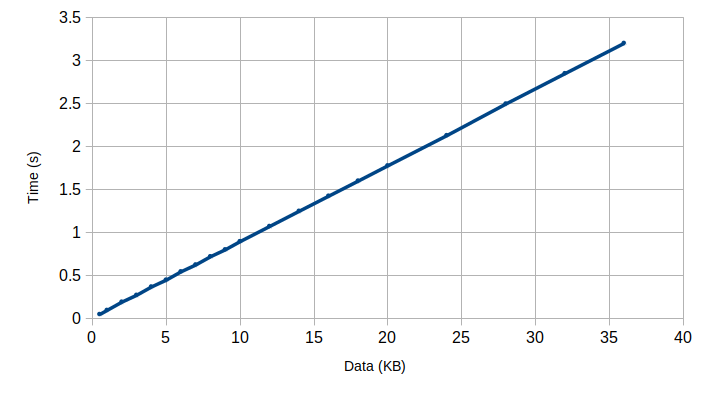
\includegraphics[width=0.8\textwidth]{./Images/comms-time.png}
	\caption{Serial Port data transmission times}
	\label{fig:comms:time}
\end{figure}

For the subsequent graphic, the throughput was calculated from the transmission tests, for every repetition.
Figure~\ref{fig:comms:tput} plots the experimental throughput and theoretical throughput. The theoretical throughput was calculated from the baud rate \(115200/8 = 14.06 KBytes/s\).
We observe the experimental throughput starts at around 10 KB/s for smaller data sizes and stabilizes around 11 KB/s as data size increases.
We can conclude the practical throughput is close to the theoretical, and as expected stabilizes as the data size increases.

\begin{figure}[h!]
	\centering
	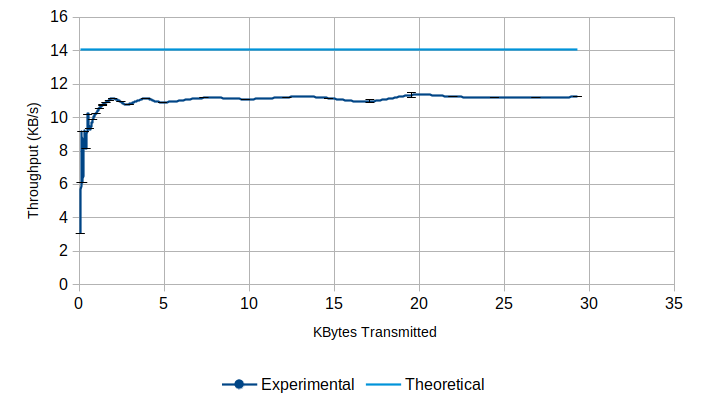
\includegraphics[width=0.8\textwidth]{./Images/comms-tput.png}
	\caption{Serial port data transmission throughput}
	\label{fig:comms:tput}
\end{figure}

% -----------------------------------------------------
% -----------------------------------------------------
\subsection{Smartfusion2 Security Services}\label{chap:evaluation:board}

All the security core accelerators of the smartfusion2 SoC were tested. This includes \ac{AES}, \ac{SHA}, \ac{HMAC}, KeyTree based \ac{SHA} and \ac{ECC} scalar multiplication and point addition.
As discussed before, all services were tested using the two presented configurations. The results of the second configuration are significantly more stable and will are presented next.
Twenty different data sizes were used in the test, from 0.5 KB to 36 KB.

The services were tested taking into account three different time components \(T_{Total} = T_{Call} + T_{Transmittion} + T_{Service}\), with the first test configuration. The call fraction is the time it takes calling the PKCS\#11 API, before any data is transmitted or the service is executed. From the results, it can be concluded this component's impact on performance is negligible, since it is almost always 0.
Predictably, the transmission time always follow the performance model studied in the previous section.
Thus, the following security core and implemented services tests focused on solely measuring the performance of the service. To get a complete conclusion of the performance of the overall system, the total service processing time can be added to the serial port time.
Regarding the time test results, all services followed a near perfect linear evolution in function of the processed data size. Thus, each accelerator's performance can be modeled with a formula composed of two different components \ref{eq:linear-eq}, a factor independent of the data being processed, present in every service call, and a component dependent on the data size.

\begin{equation}
	\label{eq:linear-eq}
	T_{Total} = T_{Constant} + T_{Data} * KB
\end{equation}
Linear regression was used to calculate these values, presented in table \ref{tab:core-model}. The median average percentage error was calculated to assess the accuracy of the calculated models for representing each service's performance. Services which receive a fixed data size such as, the \ac{ECC} and KeyTree services, only have a constant time component.

\begin{table}[h!]
\centering
\def\arraystretch{1.5}
\begin{tabular}{|c|c|c|c|c|c|c|c|}
\hline
Time (ms) & AES    & SHA    & HMAC   & TRNG   & KeyTree & ECC Add. & ECC Mult.	\\ \hline
Constant  & 0.489  & 0.498  & 0.783  & 0.368  & 1.655   & 7.204    & 545.381	\\ \hline
Data (KB) & 11.124 & 0.807  & 7.815  & 0.007  & -       & -	   & -		\\ \hline
MAE       & 0.12\% & 0.84\% & 0.13\% & 2.29\% & -       & -	   & -		\\ \hline
\end{tabular}
\caption{SmartFusion2 services time performance according to a linear model}
\label{tab:core-model}
\end{table}


All time values are presented in milliseconds, the median average percentage error represents the error of the model values compared to the real results.
The \ac{AES} service was tested with all possible variations. Namely, with 128 bit and 256 bit keys, with all four available modes, with encryption and decryption. Only one result is shown since there was no variation in all results. The chosen \ac{AES} mode, key size or encryption/decryption operation does not impact the performance positively or negatively.
Regarding the results, the higher time factor dependent of the data implicates the service time increases faster. Overall the \ac{AES} and \ac{HMAC} total service time increases faster due to this compared to \ac{SHA}, which increases significantly slower. The constant time is similar among the three services with \ac{HMAC}'s a little higher.
The error percentages are all bellow 1\%, proving the calculated models accurately represent all three services' performance.
The \ac{ECC} services are the slowest performers, particularly the scalar multiplication, each run taking more than half a second.

\begin{figure}[h!]
	\centering
	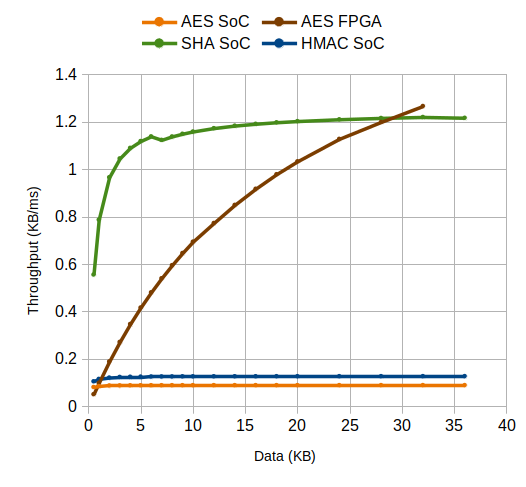
\includegraphics[width=0.9\textwidth]{./Images/core-tput.png}
	\caption{Security services throughput evolution}
	\label{fig:performance:core-tput}
\end{figure}

This graphic represents the throughput calculated from the processing time results previously gathered. The graphic shows all services throughput, shown in KB/ms, increases as the data size also increases, all eventually stabilizing at a specific value. \ac{AES} stabilizes at around 1.2 KB/ms, and both \ac{SHA} and \ac{HMAC} at around 0.1 KB/ms.

% -----------------------------------------------------
% -----------------------------------------------------
\subsubsection{Core/Software Comparison}\label{chap:evaluation:services:software}

The SHA and HMAC performance difference results were puzzling. The HMAC data dependent portion of 7.815 ms is nearly 10 times higher than the SHA value. This means HMAC time performance degrades nearly 10 times faster compared to the SHA performance. This is a surprising result since the HMAC algorithm is essentially two SHA computations, so the results were expected to be similar.
For this reason, a lightweight implementation of HMAC, SHA and AES was included in the board for comparison. The library used for HMAC and SHA is \cite{ogayHMAC}, and for AES \cite{tinycrypt}. 

\begin{figure}[h!]
	\centering
	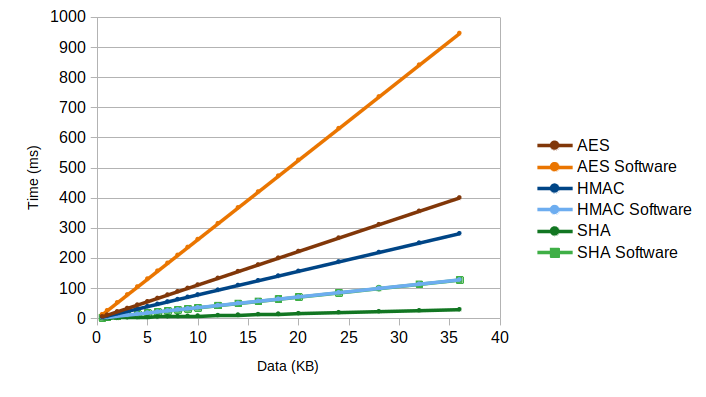
\includegraphics[width=0.9\textwidth]{./Images/software-core-time.png}
	\caption{Performance comparison of board's cores to a software implementation}
	\label{fig:performance:software-core-time}
\end{figure}

Analysing the time performance results in figure \ref{fig:performance:software-core-time}, as expected, the SHA and HMAC software results are almost identical, the HMAC is only a slightly worse performer. Compared to the core results, the SHA core is significantly faster, and deteriorates very slowly as data size increases. The opposite happens for the HMAC core. It is convincingly a worst performer compared to the software implementation, both HMAC and SHA. 
This is a incomprehensible result, as there is no clear reason for the performance degradation results. One could think it could be caused by the \ac{DPA} mitigations in place, but it would still not explain the meaningful discrepancy compared to the SHA performance, which also includes these mitigations.
The AES software implementation was tested with a 256 bit key in CBC mode. As expected it performs worse than the core service.

% -----------------------------------------------------
% -----------------------------------------------------
\subsubsection{Memory Performance}\label{chap:evaluation:services:memory}

\begin{table}[h!]
\centering
\def\arraystretch{1.5}
\begin{tabular}{|c|c|c|c|c|c|c|}
\hline
Time (ms) & RAM Op. & Write RAM & Read NVM & Write NVM & Fetch PUF & Enroll PUF \\ \hline
Constant  & 0.085     & 0.012     & 0.01     & 8.03      & 128.49    & 747.84  \\ \hline
Data (KB) & 0.34     & 0.014     & 0.02     & 298.10    & 0.006     & 0.008  \\ \hline
MAE       & 1.90\%    & 2.76\%    & 3.76\%   & 0.31\%    & 0.17\%    & 0.06\%  \\ \hline
\end{tabular}
\caption{Smartfusion2 memory performance time values according to a linear model}
\label{tab:core-model}
\end{table}


% -----------------------------------------------------
% -----------------------------------------------------
\subsection{Implemented Services}\label{chap:evaluation:services}

All implemented services from chapter \ref{chap:implementation} were tested from a data size of 0.5 KB to 20 KB. Each service performance depends on the used accelerator's, among other factors such as memory access for reads and writes or additional code logic.
Four implemented services were tested, encryption and authentication, decryption and authentication, the import keys service, all three using the \ac{AES} and \ac{HMAC} accelerators, \ac{ECDSA} and \ac{ECDH}, both using the \ac{ECC} scalar multiplication accelerator and a \ac{SHA} accelerator. It is worth noting the encryption service also uses the \ac{TRNG} service to generate a random \ac{IV}.
Similarly to the previous core tests results, the time performance results evolve linearly and the equation components for each service were calculated using the linear regression algorithm. The results are presented in table \ref{tab:services-model}.

\begin{table}[h!]
\centering
\def\arraystretch{1.5}
\begin{tabular}{|c|c|c|c|c|c|c|}
\hline
	Time (ms) & Encrypt Data  & Decrypt Data  & Import Keys & ECDSA & ECDH   \\ \hline
	constant  & 2.1    & 0.847  & 368.994  & 629.932 & 964.535 \\ \hline
	data      & 14.678 & 14.681 & 18.518 & 0.937 & - \\ \hline
	MAE	  & 0.10\% & 0.12\%  & 2.86\% & 0.18\% & - \\ \hline
\end{tabular}
\caption{Implemented services time values according to a linear model}
\label{tab:services-model}
\end{table}

% \begin{table}[]
% \centering
% \def\arraystretch{1.5}
% \begin{tabular}{|c|c|c|c|c|c|c|}
% \hline
% Time/Service   & Encrypt + MAC	  & Decrypt + MAC  & Import Keys & ECDSA   \\ \hline
%         constant (ms) & 29.413 & 29.413 & 0.002 & 0.138 \\ \hline
%         data (ms) & 6.704 & 6.704 & 1.942 & 1.542 \\ \hline
%         MAE \%	   & 1.032 & 1.006 & 0.127 & 1.760 \\ \hline
% \end{tabular}
% \caption{Implemented services throughput model values}
% \label{tab:services-model}
% \end{table}


Analyzing the results, both encryption/decryption and authentication services predictably have very similar values, due to being based on the same board's accelerators and \ac{AES} encryption and decryption having no discernible performance difference.
There is however a detectable difference in the constant component, which is most likely due to the random \ac{IV} generation with the board's \ac{TRNG} on the encryption service, whereas in the decryption is not present.
The data dependent value, of both services, is extremely close to the sum of the previously calculated values of \ac{AES} and \ac{HMAC}, \(11.124+7.815=18.939\approx18.953\approx18.946\).
The import keys service was tested until 5 KB because of the \ac{HSM}'s '\ac{RAM} limitations, more demanding than other operations due to keys being storage in the same memory as the code. With 5 KB of key storage available, the system can store up to 20 symmetric keys of 32 bits, used to secure communications. However this can be bypassed by storing the keys in a high capacity external storage connected to the device. The keys are stored encrypted with internal keys, so they are secure.
The key generation with \ac{ECDH} and \ac{SHA}-based KeyTree derivation function performs at a constant 964.535 ms. The most demanding services is the scalar multiplication which takes half a second, and importing the key to memory, using the import keys service.
\ac{ECDSA} values increase very slowly with increasing data sizes, with a similar value to the \ac{SHA} result. The biggest impact on performance is on the constant value from scalar multiplication.
The median average percentage error for the encryption/decryption and MAC and \ac{ECDSA} are models is below 0.19\%, so the models almost perfectly represent the performance. The import keys service model has the highest error with 2.86\%, due to its nearly constant behaviour for lower data size values. From 0.5 KB to 2 KB it takes a constant 386 ms, and from there starts to increase linearly.

\begin{figure}[h!]
	\centering
	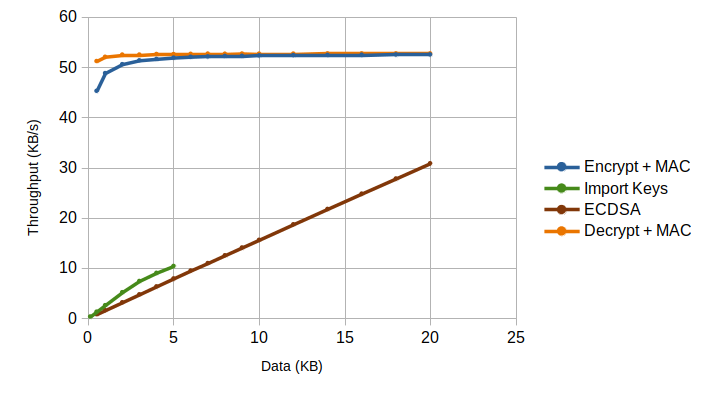
\includegraphics[width=0.9\textwidth]{./Images/services-tput.png}
	\caption{Implemented services throughput evolution}
	\label{fig:performance:services-tput}
\end{figure}

Figure \ref{fig:performance:services-tput} plots the results for throughput (KB/s) for the implemented services.
Encrypt/decryption and MAC services' throughput stabilizes at around 68 Kb/s, while \ac{ECDSA} and key importation present a somewhat linear scalability as data size increases.

\begin{figure}[h!]
	\centering
	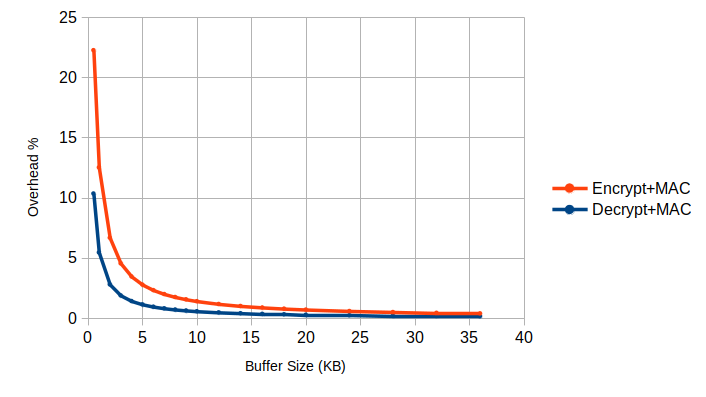
\includegraphics[width=0.9\textwidth]{./Images/buffer-overhead.png}
	\caption{Implemented services throughput evolution}
	\label{fig:performance:buffer-overhead}
\end{figure}


% TODO
% The results in table~ for the encryption and decryption operations are very similar due to both using the same board services, AES encryption and HMAC, but in a different order. It is also important to note AES encryption and decryption in CTR mode is essentially the same operation due the mode's characteristics.
% Relating to the variation in data size, the values vary between approximately 0.1284 and 0.1825 seconds, which is a very insignificant difference. Thus we can conclude, the data size has a negligible impact on the operations performance.

% TODO
% Regarding the key generation operation results in table~, two values were obtained through different methods. Due to the operation using SRAM-PUF services to enroll new keys in the eNVM memory, with limited write cycles and key slots, this operation cannot be repeated enough times to get a relevant enough sample size.
% So a trade off was achieved. The operation was performed 1000 times without the key enrollment operation, meaning only the ecdh key generation algorithm and key derivation function (SHA-256).
% Since the enrollment phase is presumed to be expensive, due to writing in eNVM memory, the test was also performed 10 times with key enrollment, to get an idea of its potential performance cost.

% This result is congruent with the one obtained by \cite{parrinha2017flexible} of 0.57s per ECC scalar multiplication.

% -----------------------------------------------------
% -----------------------------------------------------
\section{Requirements}\label{chap:evaluation:requirements}

The smartfusion2 SoC is a portable HSM which can be assigned to individuals.
The secure data exchange allows communications between individuals or groups of individuals.
The system handles all operations, the user does not have unnecessary responsibilities.
The device has physical anti-tampering measures and the communications are secured with the data exchange service.
The system also allows communications with new entities with similar devices.
It provides a easy-to-use interface software for the user's computer, using the PKCS\#11 standard to increase device interoperability.
Compared to the available HSM's on the market, the device is one of the cheapest, a M2S090TS smartfusion2 evaluation kit is priced at 384 € \cite{smartfusionPrice}.

% ------------- Requirements ------------------
% Devices should be distributable to individuals or entities with one or more individuals;
% The system must allow communications between individuals representing themselves or an entity;
% The system must be responsible for securing all communications against any sort of attacks;
% The device should be independent from user's personal computers;
% Users should be able to create secure communications with available and new entities;
% m New secure connections should be created, if existing communications are suspected to be compromised;
% It should provide an easy-to-use interface by everyone, including non-technical people;
% It should have a relatively low cost, to allow distribution of several devices among multiple people;
% Only authorized individuals should be able to use the device.
% -----------------------------------------------------
% In order to secure communications, the following services must be guaranteed: confidentiality, integrity and authentication.
% With asymmetric keys the system can provide non-repudiation to documents or files, by means of qualified digital signatures.

% -----------------------------------------------------
% The device must store all keys related to the entity who owns the device.
% The device must support secure storage in order to store the user's sensitive information, such as the cryptographic keys.
% These keys must never be exposed to the outside environment of the device to ensure the security of communications and independence of the system.
% All cryptographic operations must also be performed inside the device.
% Additionally, the device should have physical tamper-resistant measures and mechanisms in place, in case of an intrusion, such as, permanent erasure of all sensitive data.
% This means that even if an attacker is in possession of the physical device, it should be extremely difficult or even impossible to extract any information from it.
% -----------------------------------------------------
% The solution should work with a plethora of devices, which will increase the adoptability of the solution among clients.
% The system should provide an application on the user's device, which will communicate with the physical device, and make the operation's available to the user through a simple interface for the regular non-tech savvy user.
% Another related requirement is the usage of a common connection solution, e.g. \ac{USB} cable, to further increase the pool of supported devices.
% In addition, the system should perform the operations in a reasonable time to minimize the user's wait, and improve the user experience.
% ---------------------------------------------

% secure comms - aes and hmac services are not dpa resistant, so keys should be regularly replaced to avoid enough data which enables an attacker to break encryption. On the other hand this is only possible if the attacker has physical access to the device or potentially with some type of malware on the user's computer.
% key generation - needs assymetric keys to generate new keys with public keys and salt traded beforehand - can be not user friendly

% -----------------------------------------------------
% -----------------------------------------------------
\section{Summary}\label{chap:evaluation:summary}
